\documentclass[11pt,letter]{article}
% \include{macro-file}

\def\mainroot{ell_1}

%%%%%% Margins and spacing
\usepackage[top=1in, bottom=1in, left=1in, right=1in]{geometry}
\usepackage{algorithm}
\usepackage{amsmath}
\usepackage{url}
\usepackage{caption}
\usepackage[compact]{titlesec}
%\usepackage{bm}
\usepackage{txfonts} %\usepackage{times}
\usepackage{color}
\usepackage{tikz}
\usetikzlibrary{calc}
\usepackage{cancel}
\usepackage{soul}
\usepackage{graphicx}
\usepackage{caption}
\usepackage{subcaption}
\usepackage{algpseudocode}

\usepackage{sidecap}
\sidecaptionvpos{figure}{c}

\usepackage{enumitem}
\setlist{nolistsep}

%\setcounter{MaxMatrixCols}{20}

\newcommand\mjsnote[1]{{\bf [#1 -mjs]}}

\newcommand{\meas}{{\mathbf \mu}}
\newcommand{\tightpgh}[1]{\vskip 3pt\noindent\textbf{#1}}
\newcommand{\signalw}{{\mathbf w}}
\newcommand{\signalx}{{\mathbf x}}
\newcommand{\signaly}{{\mathbf y}}
\newcommand{\signalz}{{\mathbf z}}

%\expandafter\def\expandafter\normalsize\expandafter{%
%    \normalsize
%    \setlength\abovedisplayskip{2pt}
%    \setlength\belowdisplayskip{2pt}
%    \setlength\abovedisplayshortskip{0pt}
%    \setlength\belowdisplayshortskip{0pt}
%}\makeatother
%
%\renewcommand\floatpagefraction{.9}
%\renewcommand\topfraction{.9}
%\renewcommand\bottomfraction{.9}
%\renewcommand\textfraction{.1}   
%\setlength{\textfloatsep}{10pt plus 1.0pt minus 2.0pt}
\usepackage{xcolor}
\definecolor{pykeyword}{HTML}{000088}
\definecolor{pyidentifier}{HTML}{000000}
\definecolor{pystring}{HTML}{008800}
\definecolor{pynumber}{HTML}{FF4000}
\definecolor{pycomment}{HTML}{880000}


\usepackage{listings}
\lstset{language=bash,
        basicstyle=\ttfamily\small,
        tabsize=4,
        showstringspaces=false,
        keywordstyle=\color{pykeyword},
        identifierstyle=\color{pyidentifier},
        stringstyle=\color{pystring},
        numberstyle=\color{pynumber},
        commentstyle=\color{pycomment}
}

% Jian \DeclareMathOperator*{\median}{median}
\newcommand{\mb}{\ensuremath\mathbf}
\newcommand{\F}{\ensuremath\mathbb{F}}

\title{UI for RNA-seq quantification \footnote{Course Project Report of CSE 549.}}
\author{
%\alignauthor
Yigong Wang\\
       {\small SBU ID: 109973706}\\
       {\small Department of Computer Science}\\
       {\small Stony Brook University} \\
       {\small \texttt{yigwang@cs.stonybrook.edu}}
%\alignauthor
\and
Hongjin Zhu \\
       {\small SBU ID: 109748818}\\
       {\small Department of Computer Science}\\
       {\small Stony Brook University} \\
       {\small \texttt{hozzhu@cs.stonybrook.edu}}
%\alignauthor
\and
Jianglin Wu \\
       {\small SBU ID: 108075432}\\
       {\small Department of Computer Science}\\
       {\small Stony Brook University} \\
       {\small \texttt{jiangwu@cs.stonybrook.edu}}
%\alignauthor
\and
%\alignauthor
Jian Yang \\
       {\small SBU ID: 110168771}\\
       {\small Department of Computer Science}\\
       {\small Stony Brook University}\\
       {\small \texttt{yang16@cs.stonybrook.edu}}
}
\date{}


\raggedbottom

\begin{document}
\maketitle

\begin{abstract}
RNA sequencing, is a technology that uses the capabilities of next-generation sequencing to reveal a snapshot of RNA presence and quantity from a genome at a given moment in time. There are many modern algorithms for RNA-seq but there is few visualization about the algorithms' results. Based on this status, we implemented a UI for RNA-Seq quality comparison between various of algorithms. The UI could upload results from algorithms, generate plots and tables for quality metrics and a user could interactively view any data on the plots.
\end{abstract}

\thispagestyle{empty}
\addtocounter{page}{0}

\section {Introduction}

Software developed by programmer can process high throughput RNA-seq data and create detail results for Biologist and Bioinformatician for further analyzing. However, these tools cannot replace the role of a professional user who knows how to deal with the data and the meaning behind the number and text.  A simple graph contains more information than paragraphs of text description.  So, to provide an easy way for Biologist to research on the output data, we have our User Interface which consists of following functionalists: Bar chart for basic statistical information about the data; Scatter Plots for algorithm output data visualization, comparison and analysis; and Metrics for performance evaluation.   \\
To implement such an application, we used Python as the backend, we build a web service based on Tool Django and using JavaScript at frontend and using Python at the backend. \\
As an application, a user could view a bar chart to compare the statistics among all the statistics and also could choose any two attributes for a scatter plot. Any also a node's information could be showed as interaction. At last, a performance evaluation could be listed with the ground truth file.


\section {UI Architecture}
As a web application, this application includes the following parts as: \\
\begin{enumerate}
\item Webpage displayed at user's browser.
\item Server to accept request from a user and send the webpage and contents to user.
\item Request Handler to handle the request and query the related data from Data Layer. The result would also be packed to JSON format and send back to Server side.
\item Data Layer to load and process data.
\end{enumerate}

The Architecture is showed in figure \ref{architecture}.
\begin{figure}[h!]
\centering
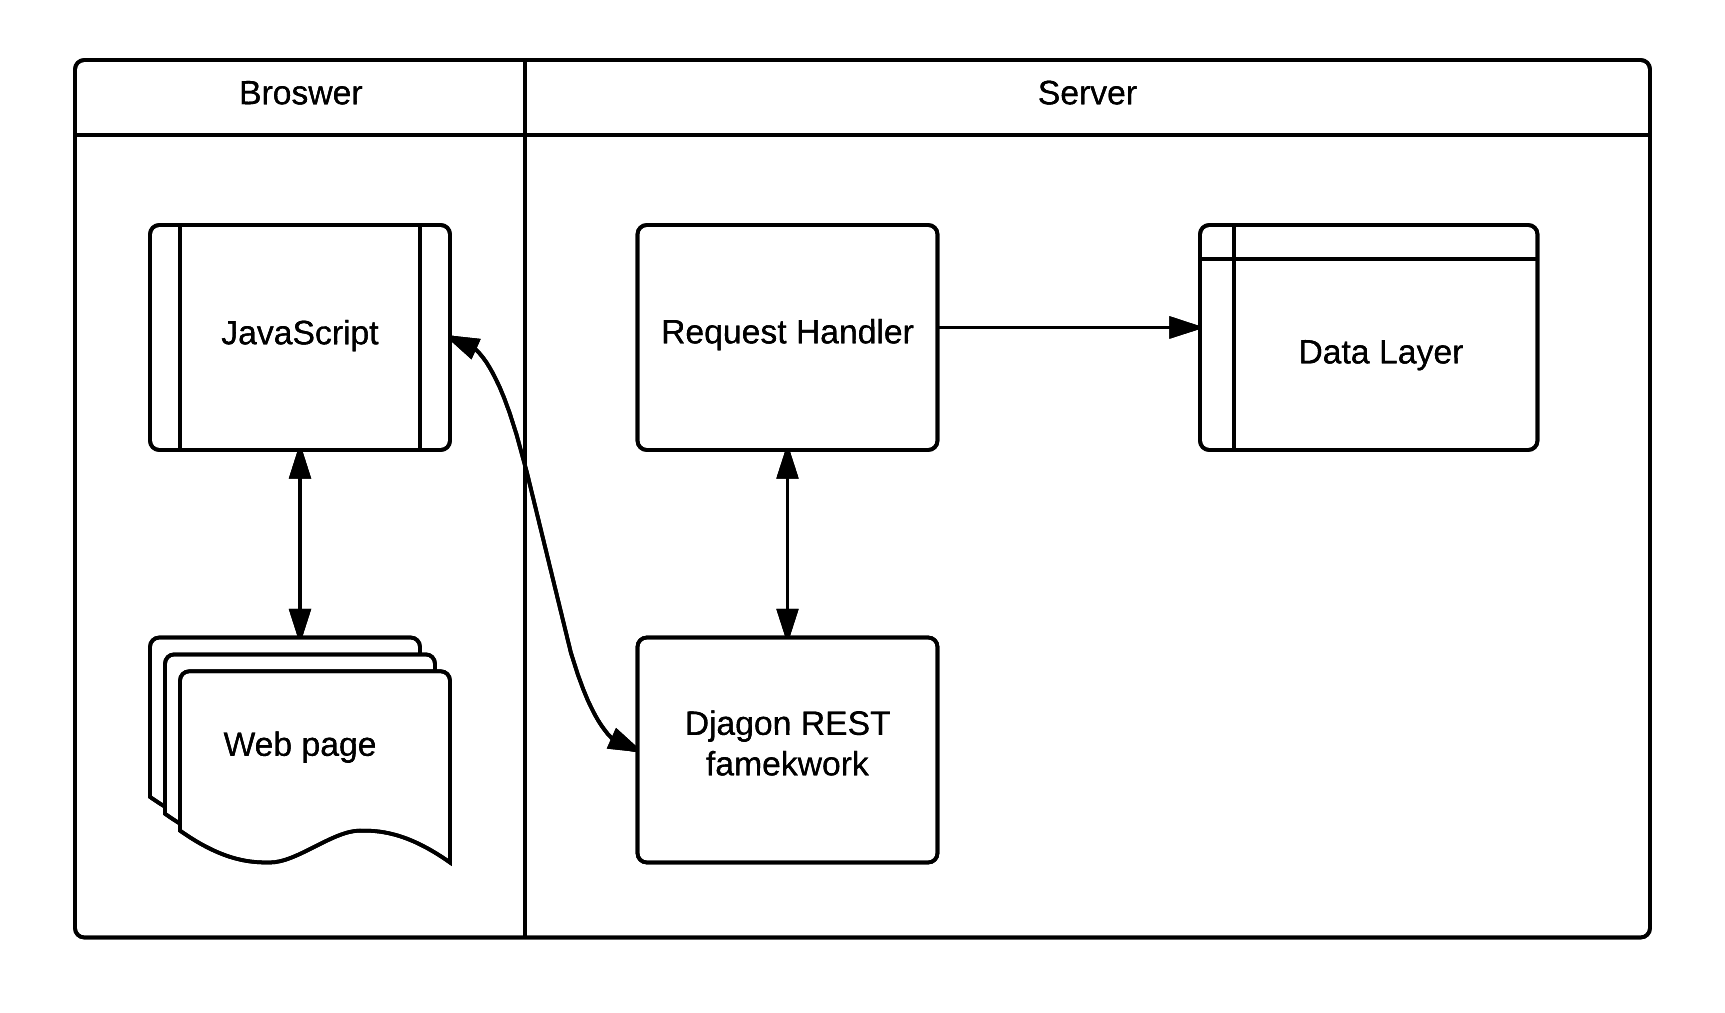
\includegraphics[height=2.5in, width=5in]{./fig/arch.png}
\caption{Architecture}
\label{architecture}
\end{figure}

As one example, here is one example story when a user wants to view the scatter plot for algorithm \emph{Sailfish} with the attributes GC content versus abundant estimate. The internal steps are:
\begin{enumerate}
\item User clicks the page for single algorithm plot.
\item A request for an algorithm list would be sent by JavaScript on webpage to Django.
\item Django passes the request to a Request Handler, and the handler would get the algorithm list and packaged the list o JSON package and send the package to Django.
\item Django passes the result to JavaScript, and JavaScript lists the algorithms in a drop down list.
\item User chooses one algorithm to display. Let's say the user clicks sailfish.
\item Same steps as 1. to 4., a request for all the attributes of algorithm sailfish is sent to backend and finally the list would be displayed on webpage.
\item User chooses two attributes from the list on webpage.
\item Same steps as 1. to 4. a request for the two attribute data would be sent and the data is sent back finally.
\item JavaScript plots the data on webpage.
\item When the user moves the mouse to any point on the plot and the information would be displayed on webpage by JavaScript.
\end{enumerate}

Here is the visualized flow for this example in figure \ref{fig:story}.
\begin{figure}[h!]
\centering
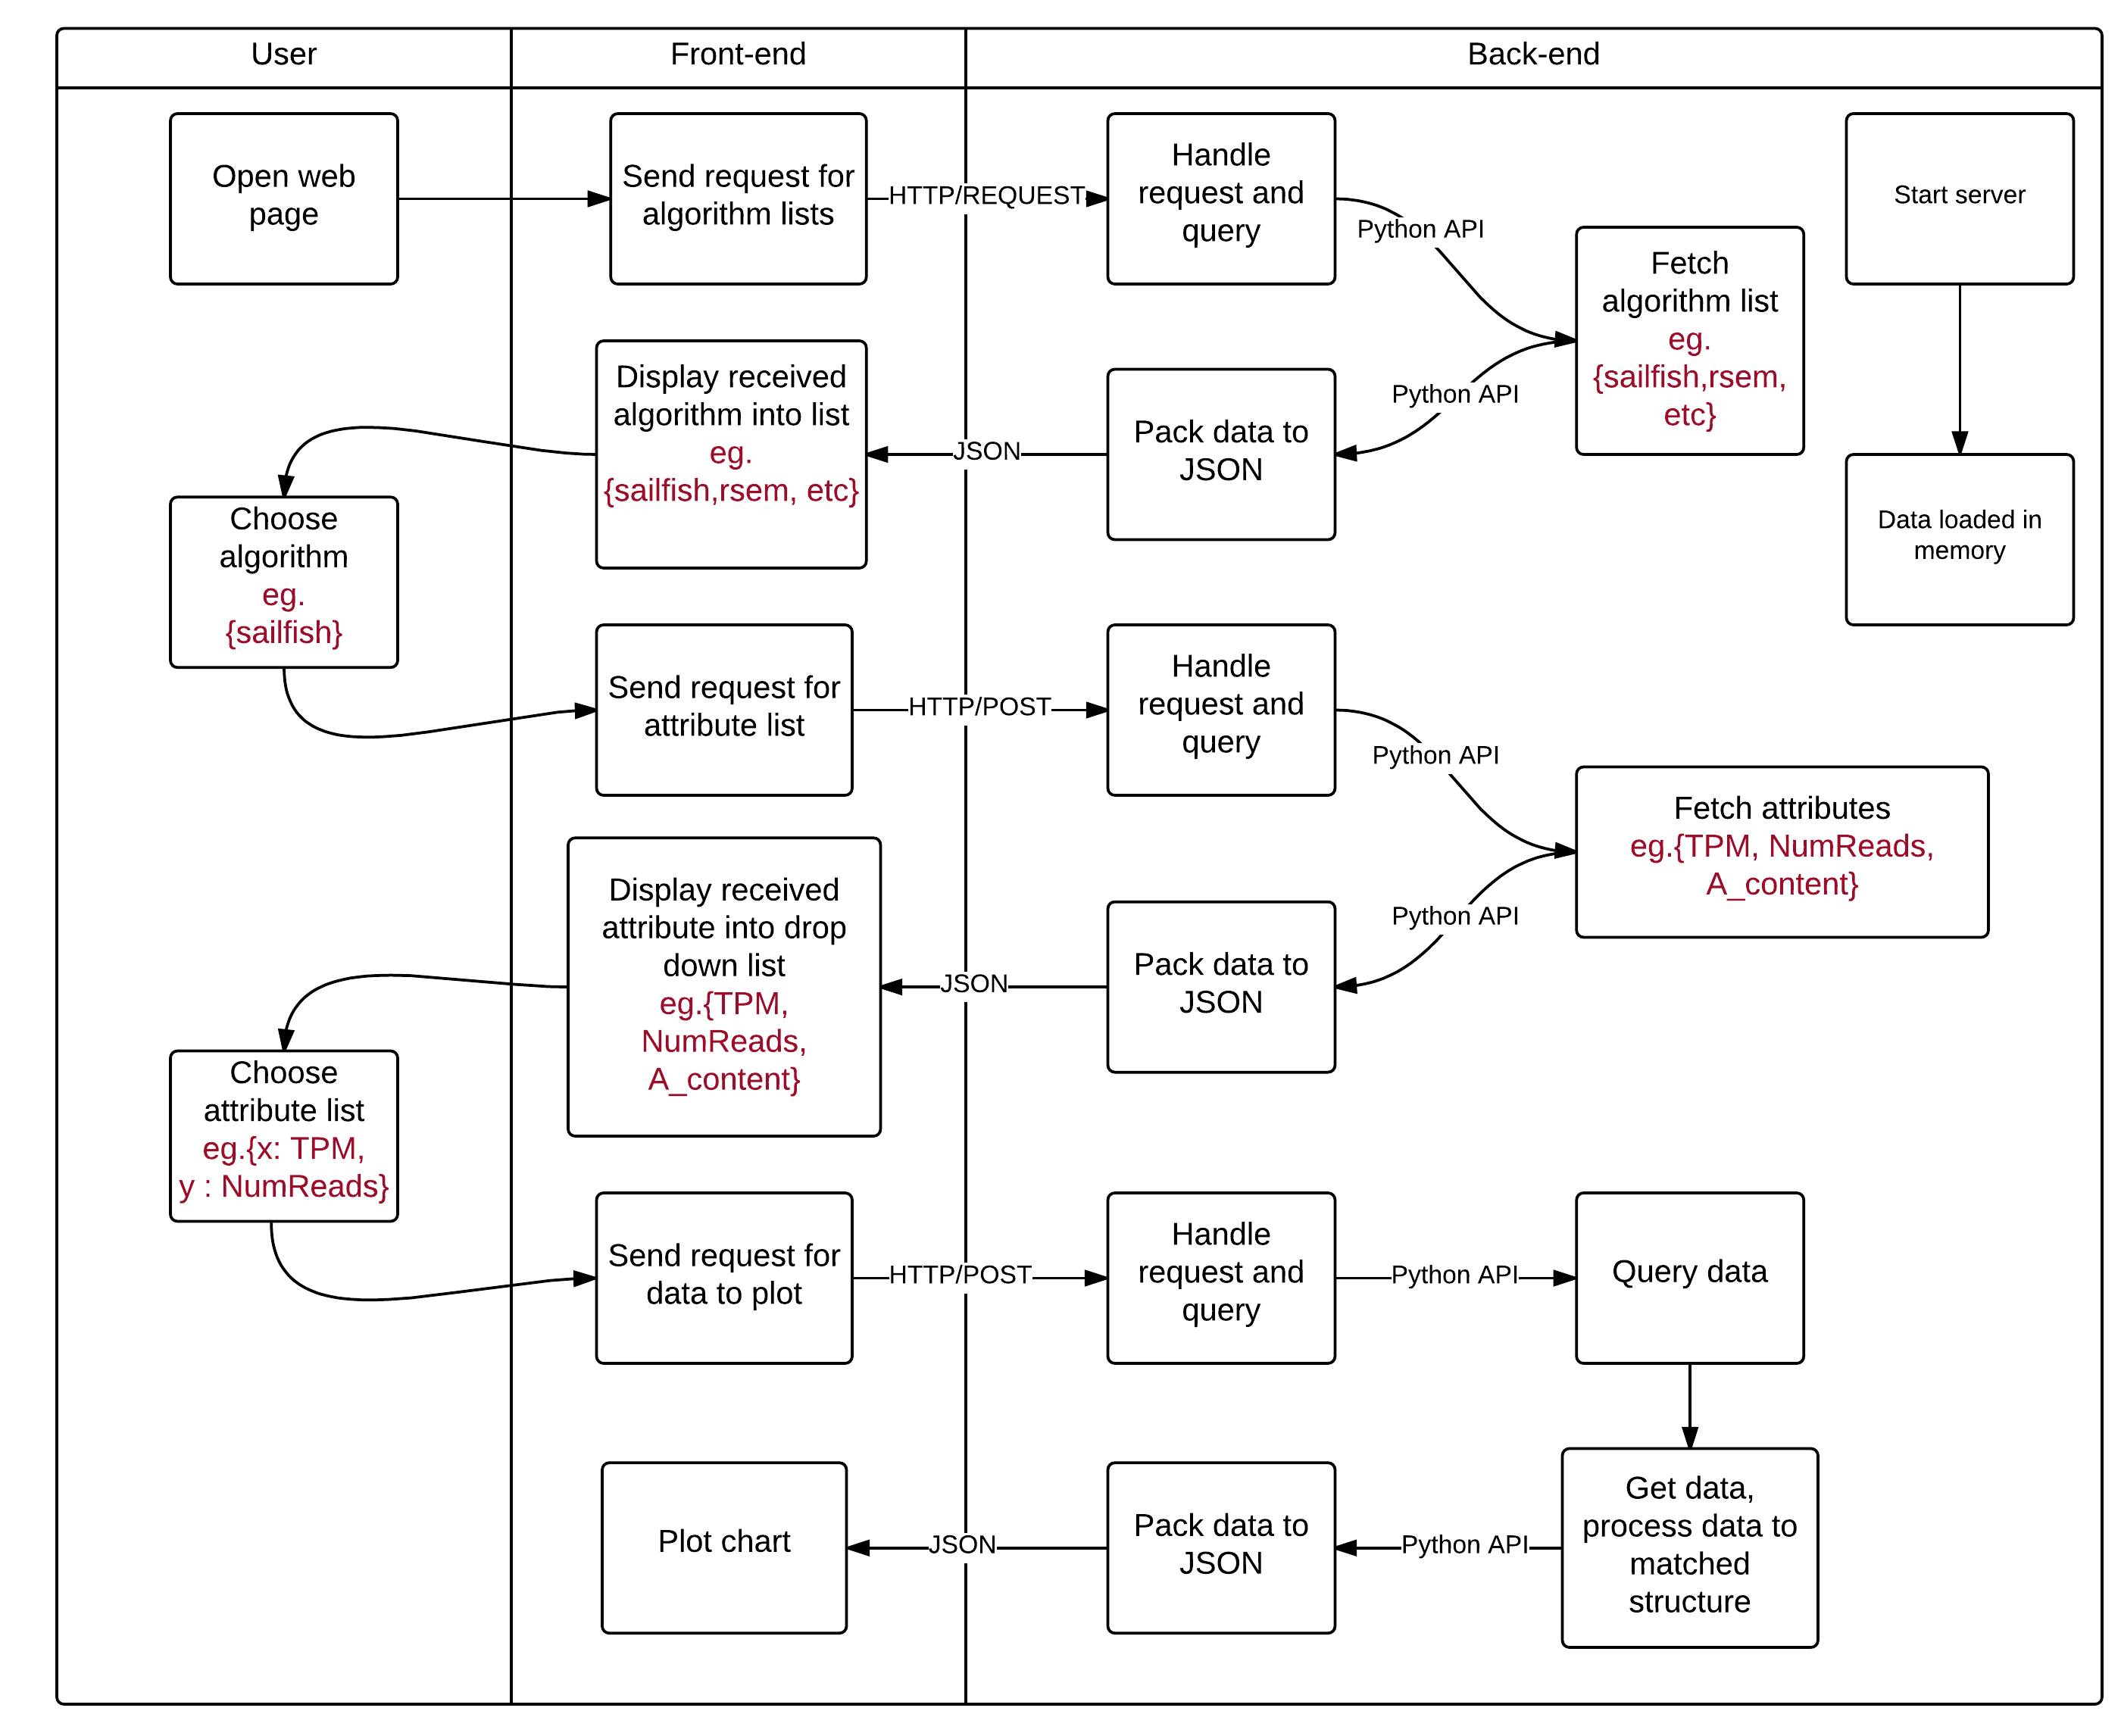
\includegraphics[height=4in, width=5in]{./fig/story.png}
\caption{Example of one request}
\label{fig:story}
\end{figure}

\section {UI Components}

\subsection {Data Layer}
At data layer scripts, we did the following jobs.
\begin{enumerate}
\item Calculate the statistics from the transcript. \\
We calculate the data such as GC content, ration of each nucleotides.
\item Load data from result files for algorithms and also the ground truth from profile files according to given parser.
\item Concat the data of results, the ground truth and the statistics based on transcript name as index to a large table.
\item Provide the API to query the algorithm list, the attributes and the data for UI layers.
\item Calculate the performance evaluation matrix.
\item Sample data if the data has too many items. \\
If there are too many data, for example, in the given data there are more than 80 thousands of points to be plotted at frontend. To reduce the size of the data and keep all the outliers, I used the following algorithm:
\begin{enumerate}
\item Calculate the centroid point of the data.
\item Calculate the distances for all points to center point and pick a distance to include 99\% of the poinrts.
\item For any points which have longer distance than the picked 99\% one, we would keep them.
\item For all points which have smaller distance than the picked 99\% boundary, we would sample them by a ratio.
By using this sample, we could get 0.5\% to 1\% size of the original data size.
\end{enumerate}
\end{enumerate}
% The API contains the following methods.

\subsection {Request Handler}
When the project runs, a simple server script listen to the specified localhost port. The Django preprocess all received requests of that port. In \emph{server/server/urls.py}, we defined the url scheme. Our scripts handling all requests according to this URL scheme, then wrap results to desired format and send to user browsers.  \\
Because we have different types of interactive charts, bar charts of algorithm comparison and a performance evaluation table, the URL scheme assigned three corresponding URLs to them. Every URL has scripts to process requests to it. \\
When user access the root URL, the server load all data to the memory and calculate all algorithm comparison charts. Instead of accessing file system, later data access will go to the memory directly, which is more faster and flexible. After that, the page redirect user to the main website page. \\
Here are the request types and how we would handle them.
\begin{enumerate}
\item For requests of the interactive charts, the URL is \emph{/get}. Because we have three types of chart plots. scripts of processing these requests defined three request types. Corresponding to single algorithm scatter chart, two algorithms scatter chart and two algorithms comparison chart.
\begin{enumerate}
\item Firstly, JavaScripts in the client request algorithm types, server scripts give algorithm names and their attributes to the client. According to different picture types, the script gives different attributes. For example, in two algorithms comparison chart, we only give common attributes which make sense for comparison.
\item Later on, this URL also response to the client requests for get attributes data, scripts return required data in JSON format to the client.
\end{enumerate}
\item For requests of the bar charts, the URL is \emph{/get\_common}. This URL provides all algorithm shared attributes in JSON format to the client. The client can use a predefined image URL scheme to load calculated images. For example, if an attribute is ?TPM?, predefined URL might be \emph{static/img/TPM\_bar.png}
\item For requests of the performance evaluation table, the URL is \emph{/matrix}. It provides the algorithms? performance data to the client.
\end{enumerate}

\subsection {Frontend}
We used and modified open source bootstrap template SB Admin 2 \cite{sb_admin_2} as our webpage, then integrated and implemented following:
\begin{enumerate}
\item Javascript public library:
\begin{itemize}
\item Jquery: jquery-1.8.3.min.js
\item D3js: d3.v3.min.js \cite{d3_scatterplot}
\end{itemize}

\item Javascript library which we implemented:
\begin{itemize}
\item chart.js:  plot all the scatter charts.
\item data.js: using Ajax call to fetch data from server.
\item dropDownList.js: using Ajax call to fetch algorithm and attribute information from server. Change drop down list dynamically based on user selection.
\end{itemize}

\end{enumerate}

Design details:
\begin{enumerate}
\item Dynamic drop list.
\begin{enumerate}
\item Using Ajax call to fetch JSON data from user, which contains all feasible algorithms and their relevant attribute.
\item Listening to user selection of algorithm, and dynamic change the attributes drop down list.
\item Get user's selections from drop down list and send request to server. Then get data to plot scatter charts
\end{enumerate}

\item There are three type of scatter charts.

\begin{enumerate}
\item Scatter Plot for a Single Algorithm. \\
Get user input from front end, send requests through Ajax call to get matched data from server. Get each node and plot them on svg using D3js.\\
Requirement input value from user: {algorithm name, x axis, y axis}
\item Scatter Plot for two Algorithms on the same metrics. \\
Get user input from front end, send requests through Ajax call to get matched data from server. Get each node and plot them on svg using D3js.\\
Requirement input value from user: {algorithm 1, algorithm 2, attribute}
\item Scatter Plot for two Algorithms on the same feature. \\
Get user input from front end, send requests through Ajax call to get matched data from server. Get each node and plot them on svg using D3js.\\
Requirement input value from user: {algorithm 1, algorithm 2, attribute}
\end{enumerate}

\item interactive with user. \\
When user mouse put on the spot from any scatter charts. It will display the name of the node, the x attribute value and y attribute value, and other information that user designed to display.

\item Input check.\\
Using Javascript to check user selections' validation. For example, user are not allowed to choose empty content and click the submit button. There will be some alert message.\\

\end{enumerate}

\section {Installation and Setup}
This project provides a web-based user interface, which allows users access it locally or remotely. In this section, we give a brief introduction of installation. \\
The project require following package/software:
\subsection {Dependencies}
\begin{enumerate}
\item Modern web browser\\
A modern web browser is required for the user interface. Because the interactive and data visualisation are highly depend on JavaScripts libraries, the latest version browser is highly recommended for better efficiency and experience.
\item Python 2.7.9 or later\\
The website framework and data processing are based on Python programming language.
\item Django\\
Django provides a basic web server, as well as a web framework. It lays between browser and data. To install Django, using the command (Please note that you might need the administrator privilege, e.g. sudo before pip command):
\lstset{language=bash}
\begin{lstlisting}[frame=single]
pip install django
\end{lstlisting}
\item django-cors-header\\
django-cors-headers library enables cross sites recourse sharing of the server.
\lstset{language=bash}
\begin{lstlisting}[frame=single]
pip install django-cors-headers
\end{lstlisting}
\item pandas, scipy, matplotlib\\
These libraries are used for data processing and bar charts plotting.
\lstset{language=bash}
\begin{lstlisting}[frame=single]
pip install pandas scipy matplotlib
\end{lstlisting}
\end{enumerate}
\subsection {Start Web Server}
To run the project, go to ‘server’ folder of the project, use following command.
\lstset{language=bash}
\begin{lstlisting}[frame=single]
python manage.py runserver 8000
\end{lstlisting}
This command will run the server and listen to localhost port 8000. Next, open a browser then navigate to http://127.0.0.1:8000/.

\section {UI Features}
We implemented the following features for the quality metrics with interactive modes to compare and view quality about algorithms. Currently we support 3 algorithms and a ground truth is added to compare the precision and the recall ratios.
\subsection {Bar Chart for algorithms}
We support the bar chart for all the algorithms to calculate the number of reads for each algorithm mapped in the experiment. One example is showed in figure \ref{fig:barchart_numreads}.

\begin{figure}[h!]
\centering
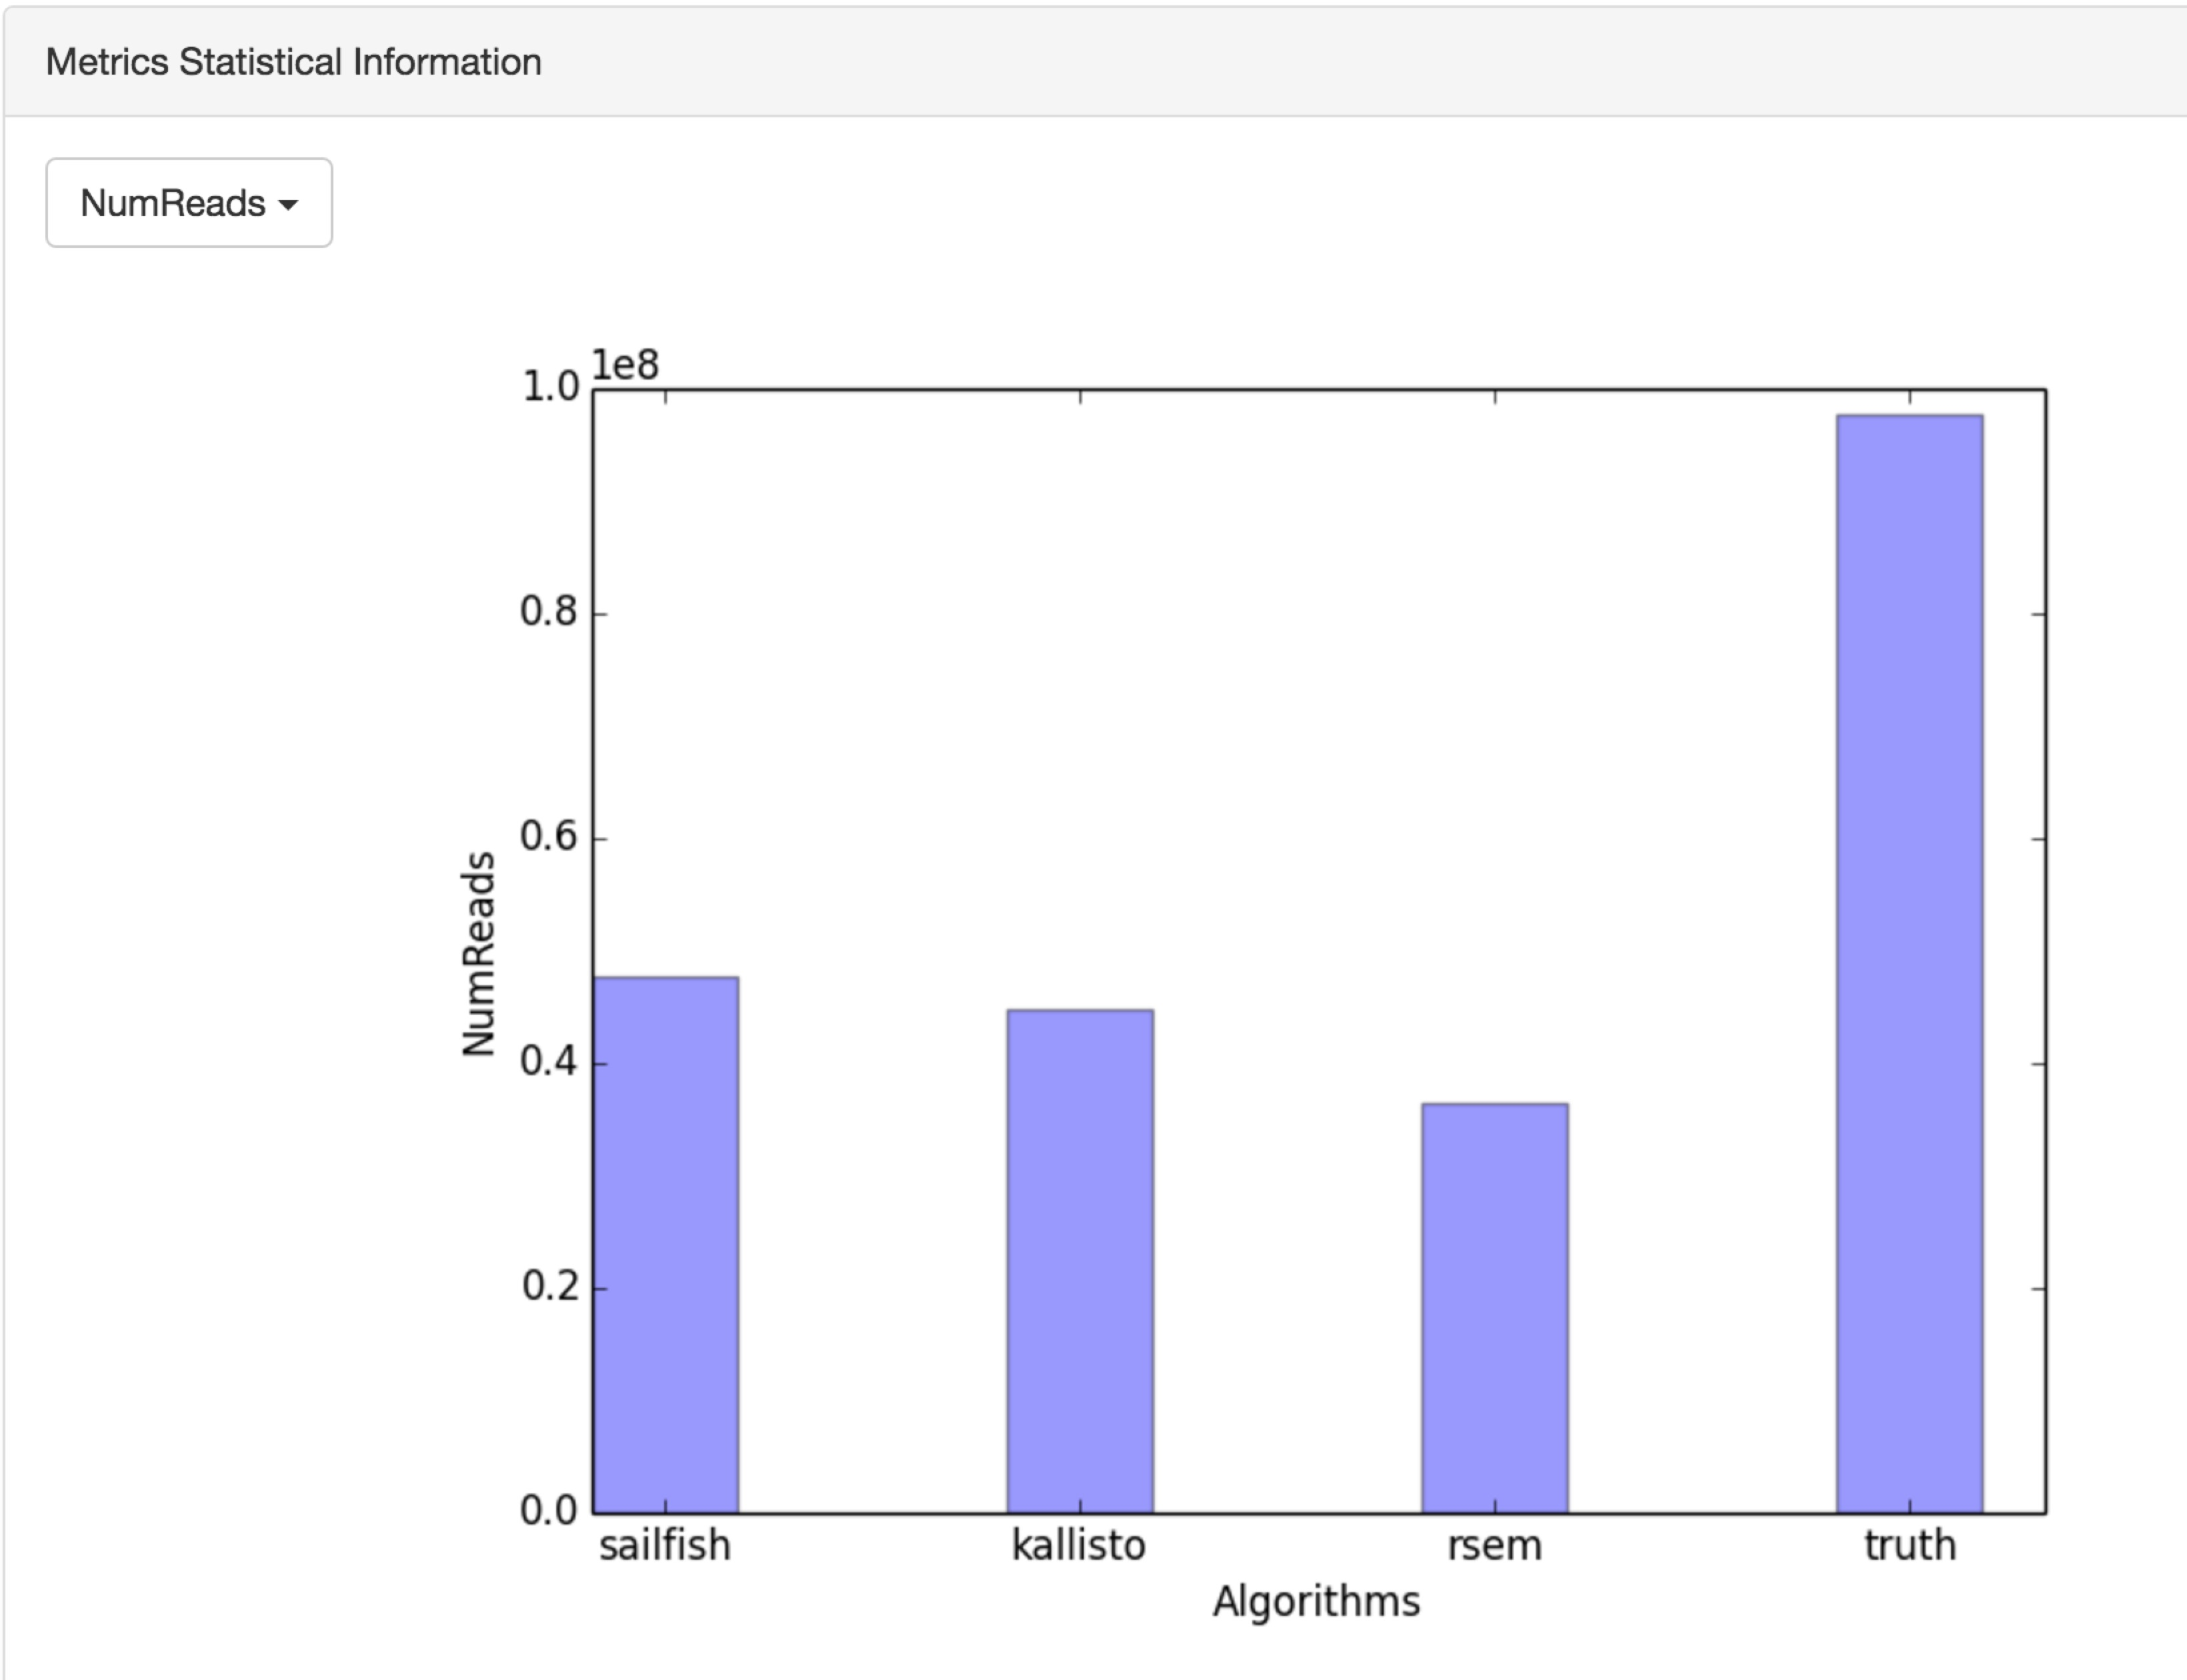
\includegraphics[height=3in, width=3in]{./fig/barchar_numreads.jpg}
\caption{Bar Chart - NumReads}
\label{fig:barchart_numreads}
\end{figure}

\subsection {Scatter Plot for a Single Algorithm}
For a single algorithm, we support the scatter plot about any two values such as transcript GC content versus abundance estimates. To plot a scatter plot, the user could go to the scatter plot for single algorithm page, choose an algorithm and the x-axis feature and the y-axis feature. With such a plot, every node on the scatter plot is one transcript and the coordinate is the chosen value pairs and as one example, the scatter plot for sailfish is showed in figure \ref{fig:single_algo_sailfish}. \\
For an interactive mode, you could move the mouse to a node you want to view and the information would automatically showed as in figure \ref{fig:interactive_single_algo_sailfish}.

\begin{figure}[h!]
        \centering
	\begin{subfigure}[h]{0.5\textwidth}
                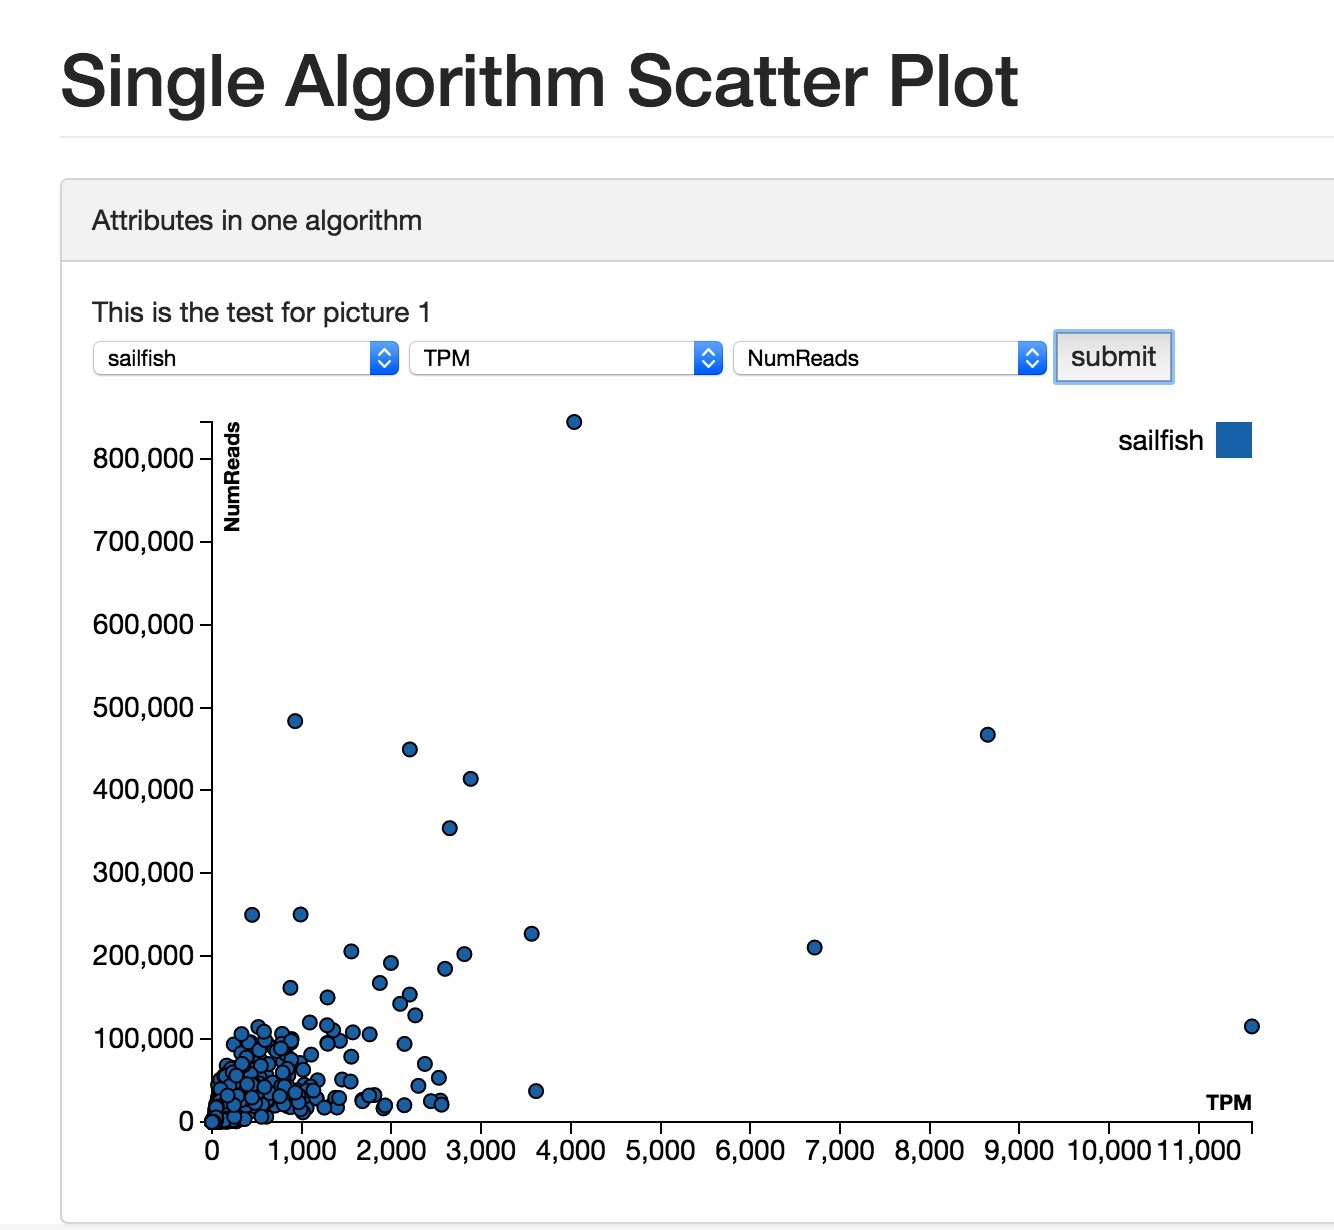
\includegraphics[height=2.5in, width=2.5in]{fig/single_algo_sailfish.jpg}
		\caption{Sailfish - NumReads vs Abundant Estimate}
                \label{fig:single_algo_sailfish}
        \end{subfigure}%
        \begin{subfigure}[h]{0.5\textwidth}
                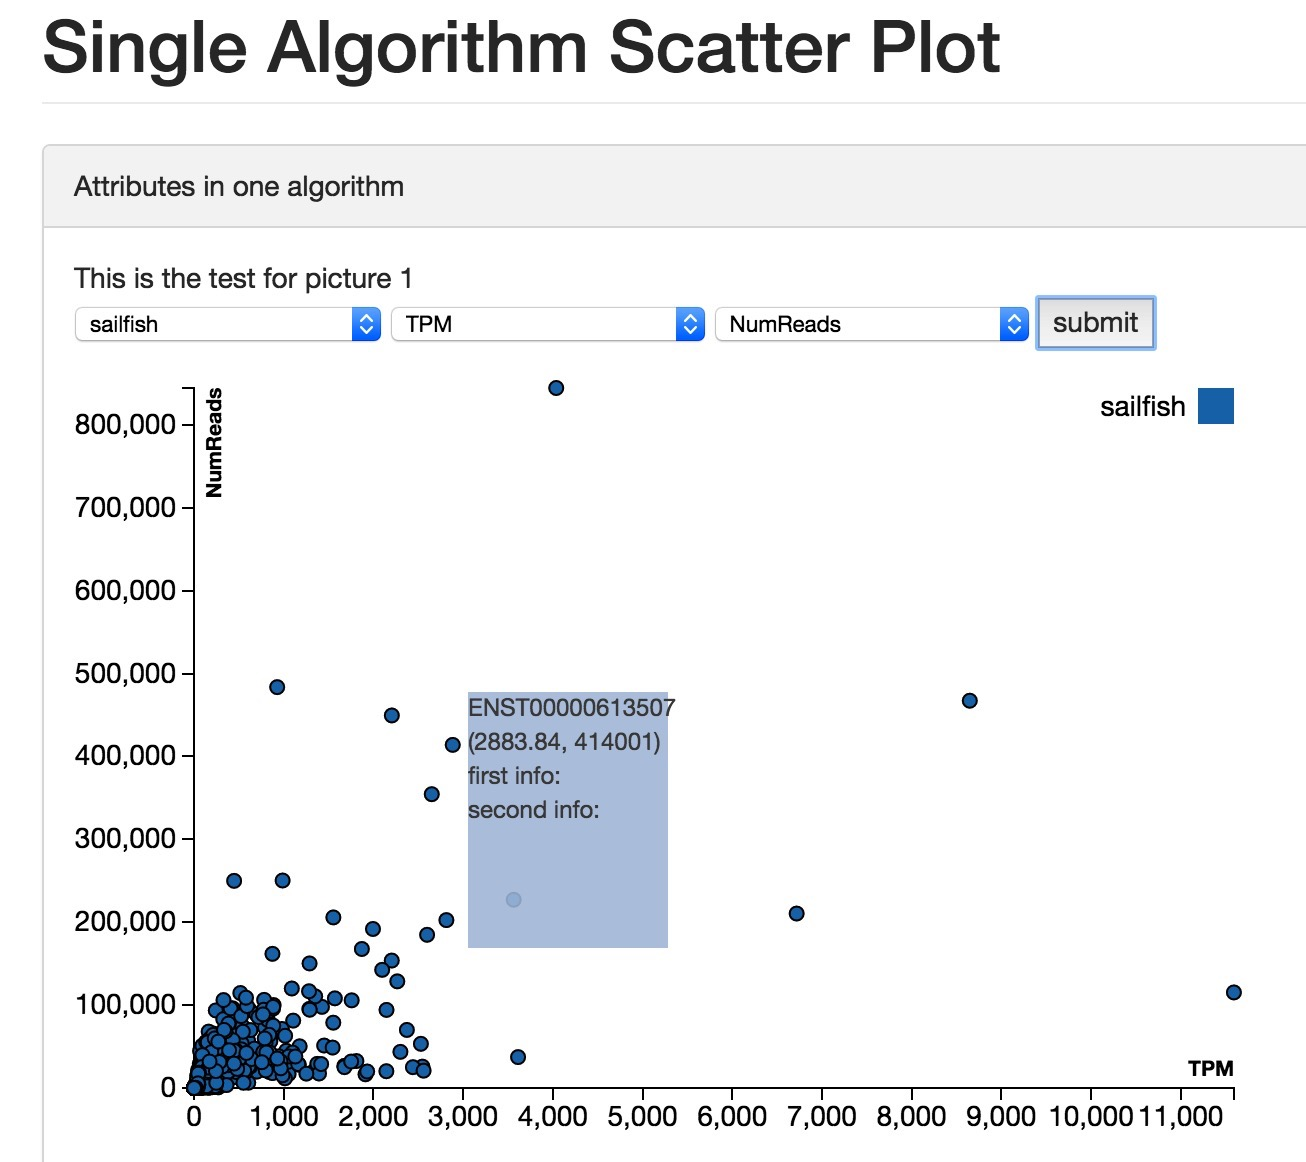
\includegraphics[height=2.3in, width=2.3in]{fig/interactive_single_algo_sailfish.jpg}
                \caption{Sailfish - NumReads vs Abundant Estimate (Interactive)}
                \label{fig:interactive_single_algo_sailfish}
        \end{subfigure}
        \caption{Pictures of Clustering with Random Sampling}\label{fig:cluster}
\end{figure}


\subsection {Scatter Plot for two Algorithms on the same metrics}
We could also compare two algorithms based on the same scatter plots. For example, we could compare the distribution between GC Content and Number of Reads for both Sailfish and Kallisto, as showed in figure \ref{fig:two_algo}.

\begin{figure}[h!]
\centering
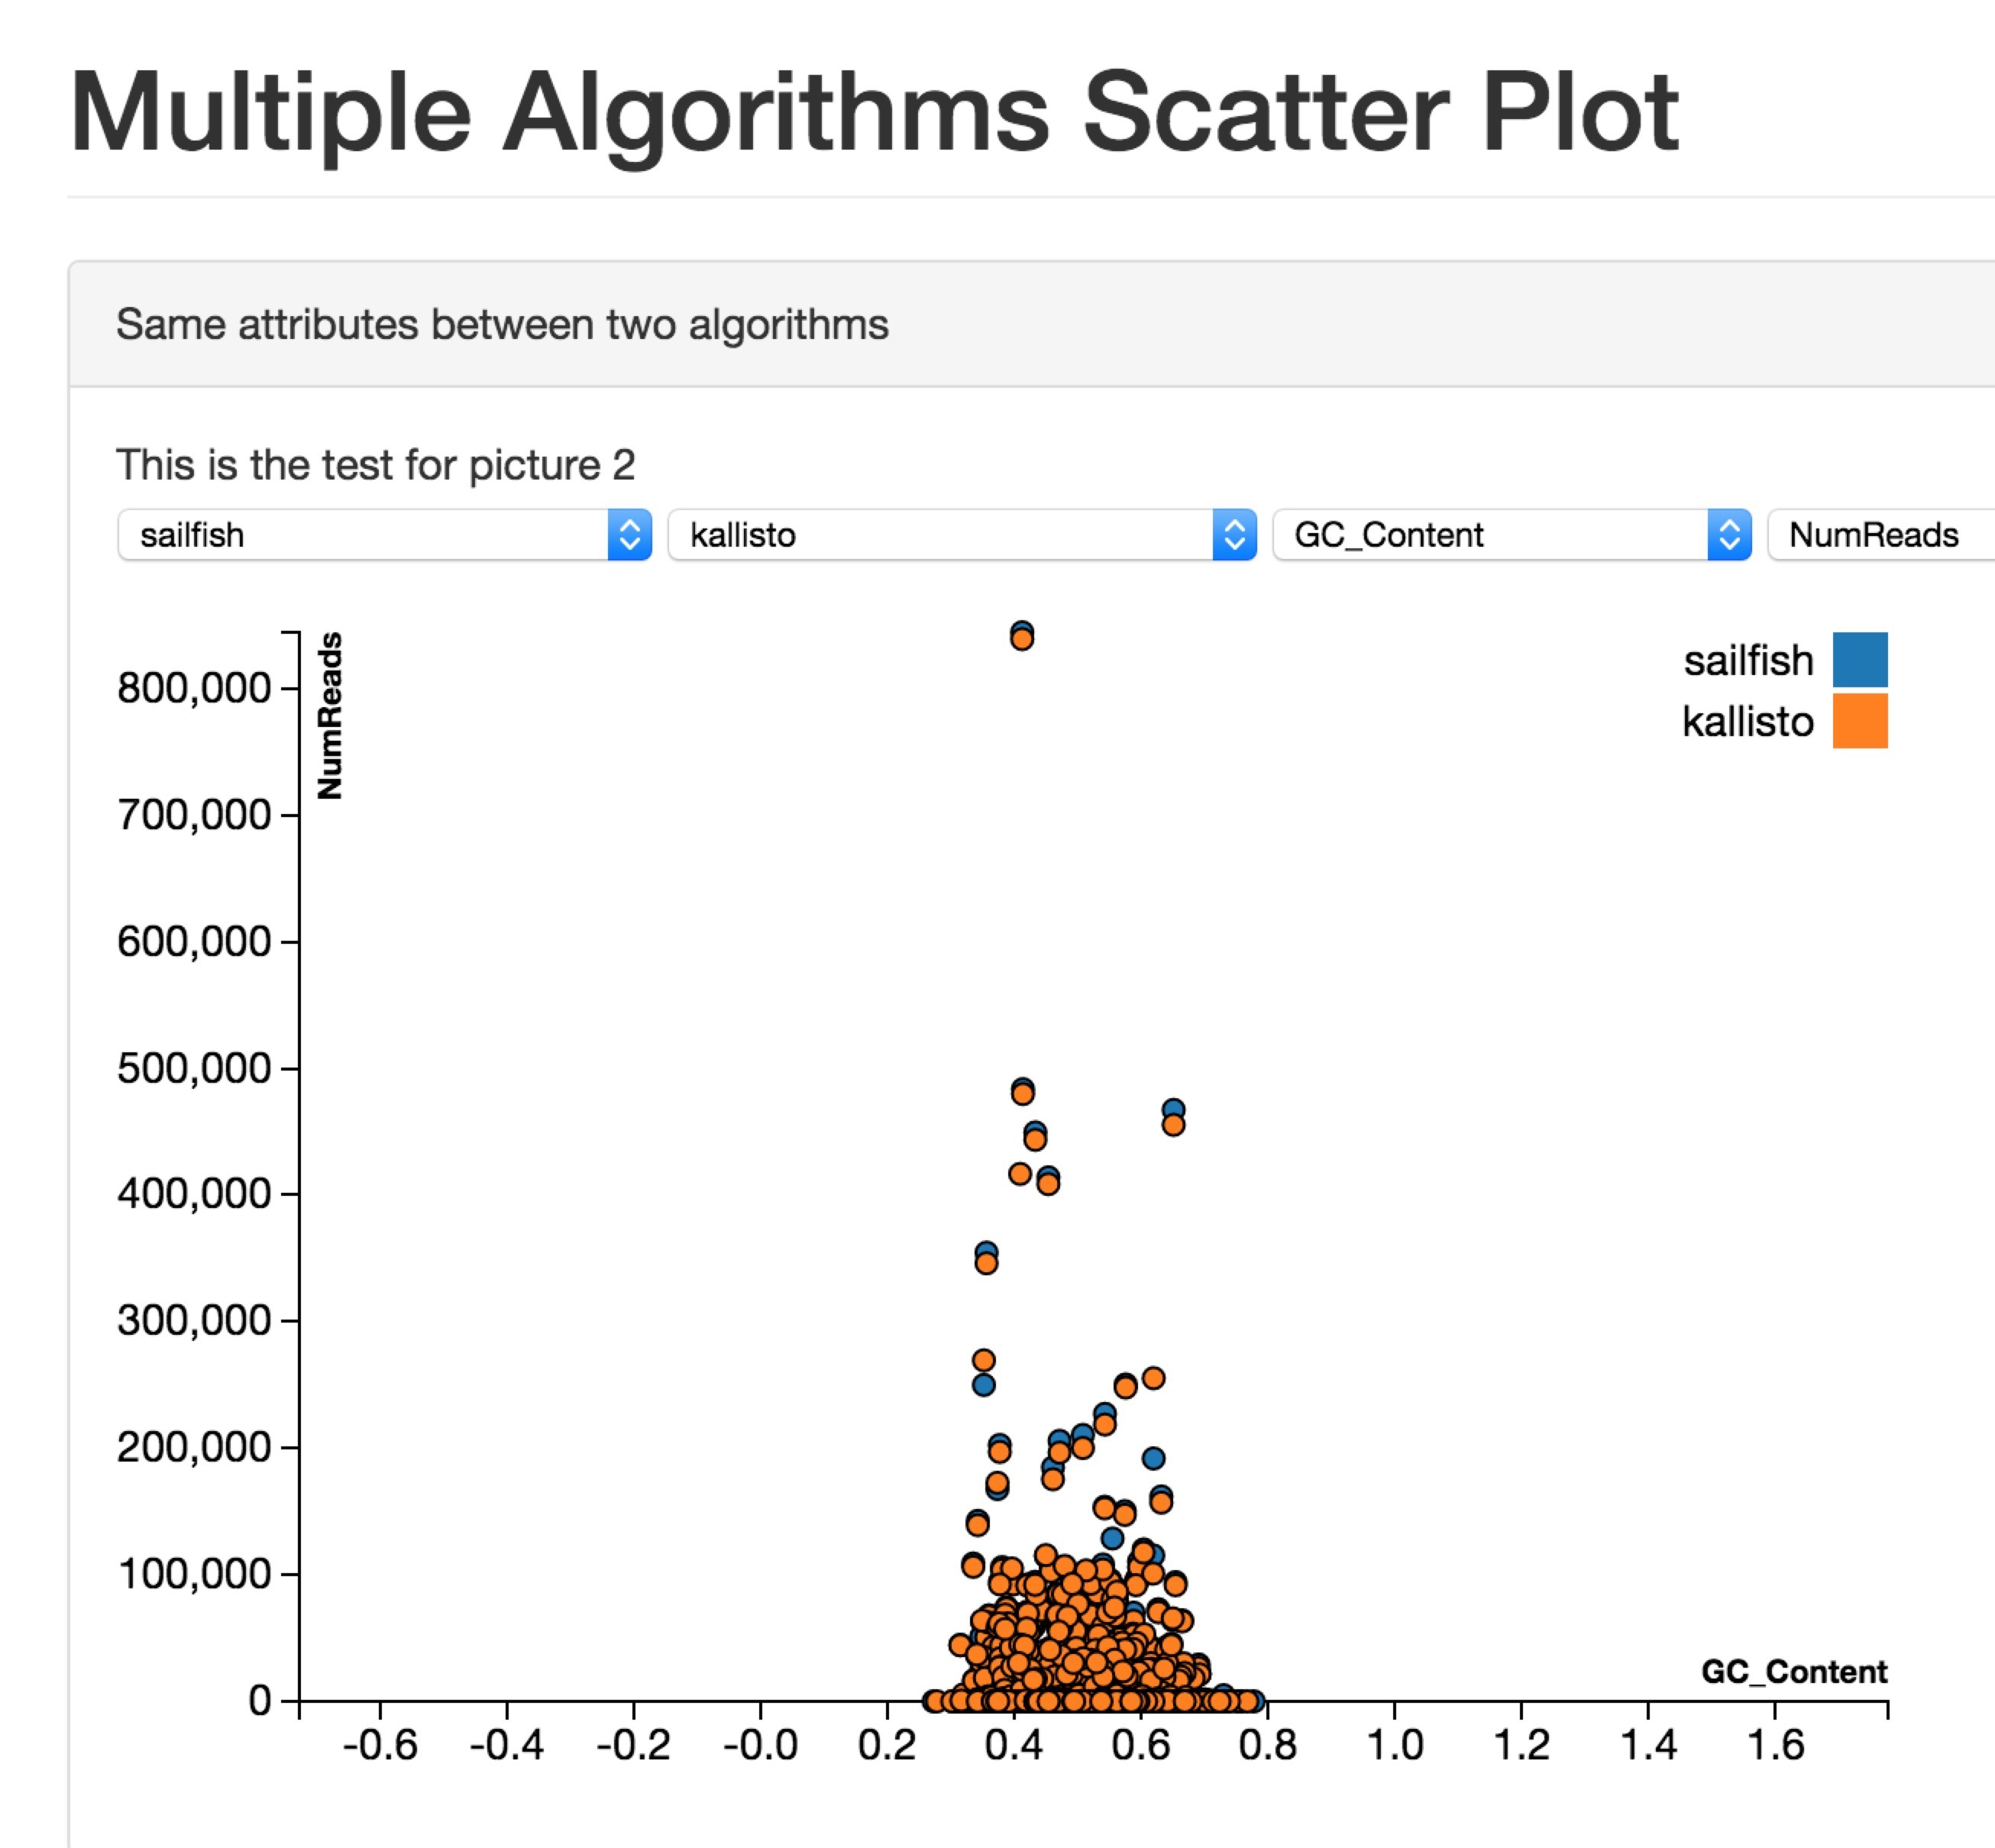
\includegraphics[height=3in, width=3in]{./fig/two_algo.jpg}
\caption{Sailfish and Kallisto:  GC Content vs  NumReads}
\label{fig:two_algo}
\end{figure}

\subsection {Scatter Plot for two Algorithms on the same feature}
The same features from two algorithms are also comparable. For example, Number of Reads for both Sailfish and Kallisto. We expected they are similar if both of them are good algorithms (figure \ref{fig:compare_sk}). And we could also compare it with the ground truth (figure \ref{fig:compare_truth}).

\begin{figure}[h!]
        \centering
	\begin{subfigure}[h]{0.5\textwidth}
                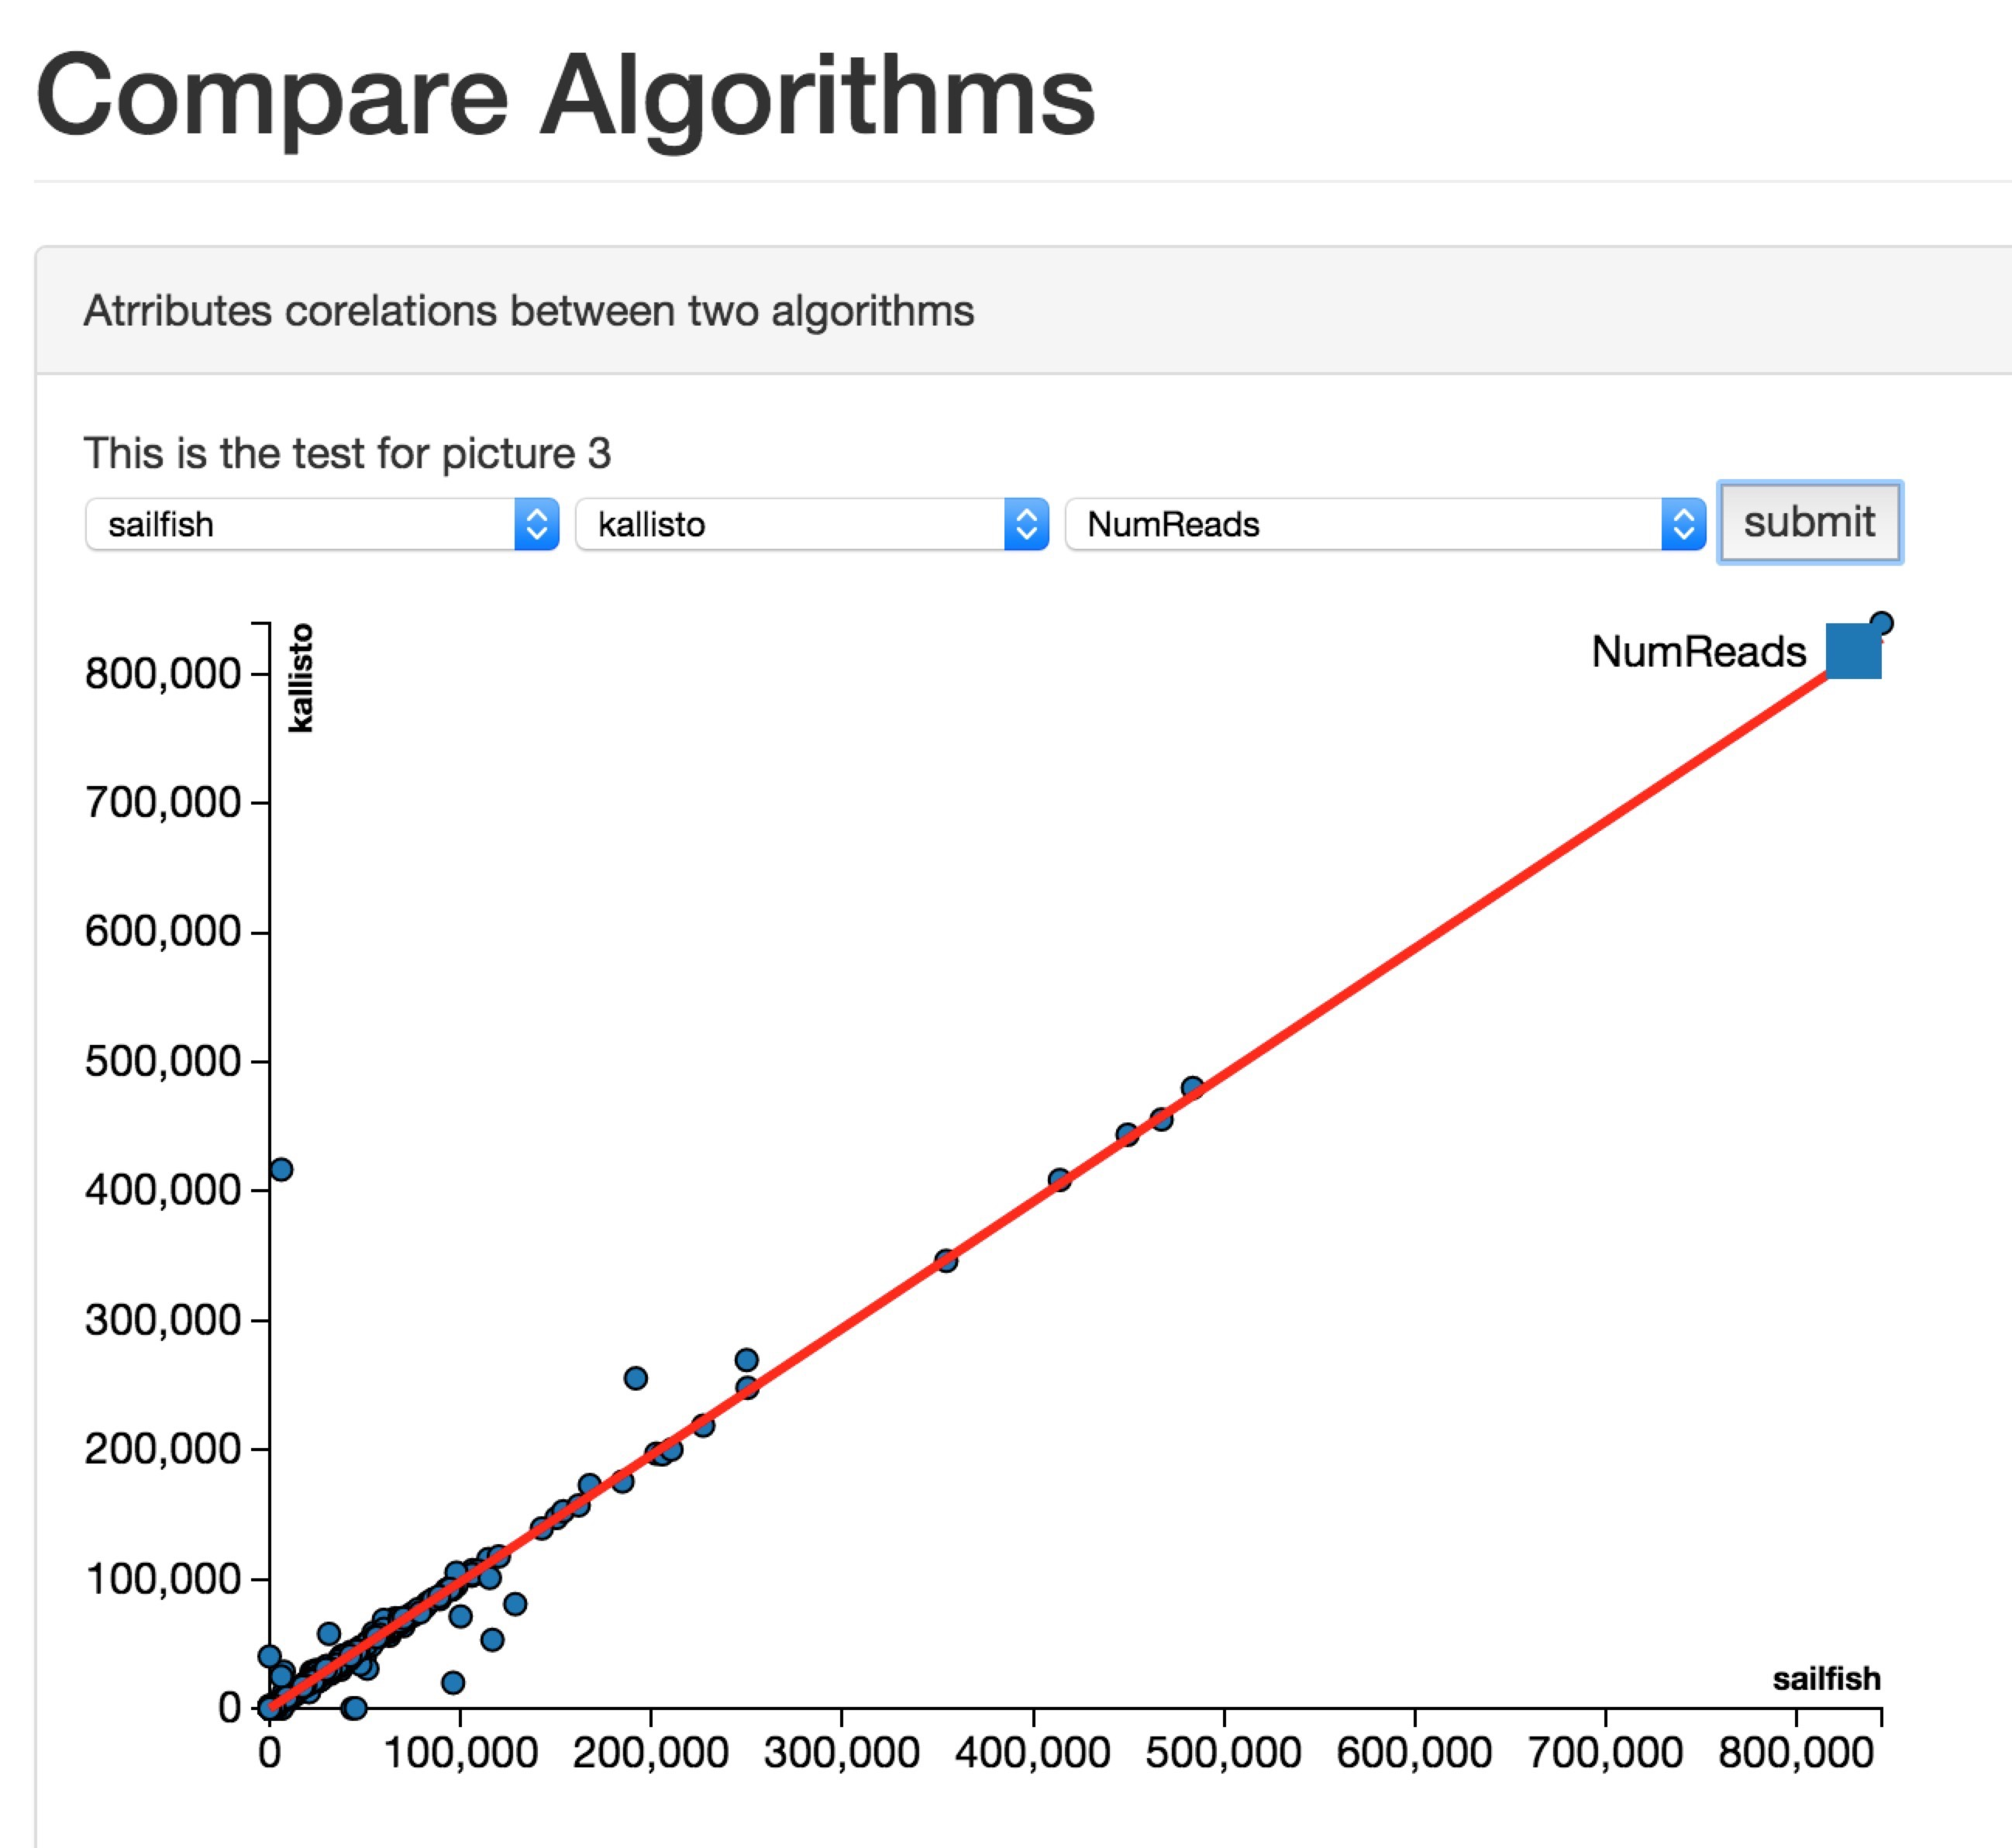
\includegraphics[height=2.5in, width=2.5in]{fig/compare_sk.jpg}
		\caption{Compare NumReads between Sailfish and Kallisto }
                \label{fig:compare_sk}
        \end{subfigure}%
        \begin{subfigure}[h]{0.5\textwidth}
                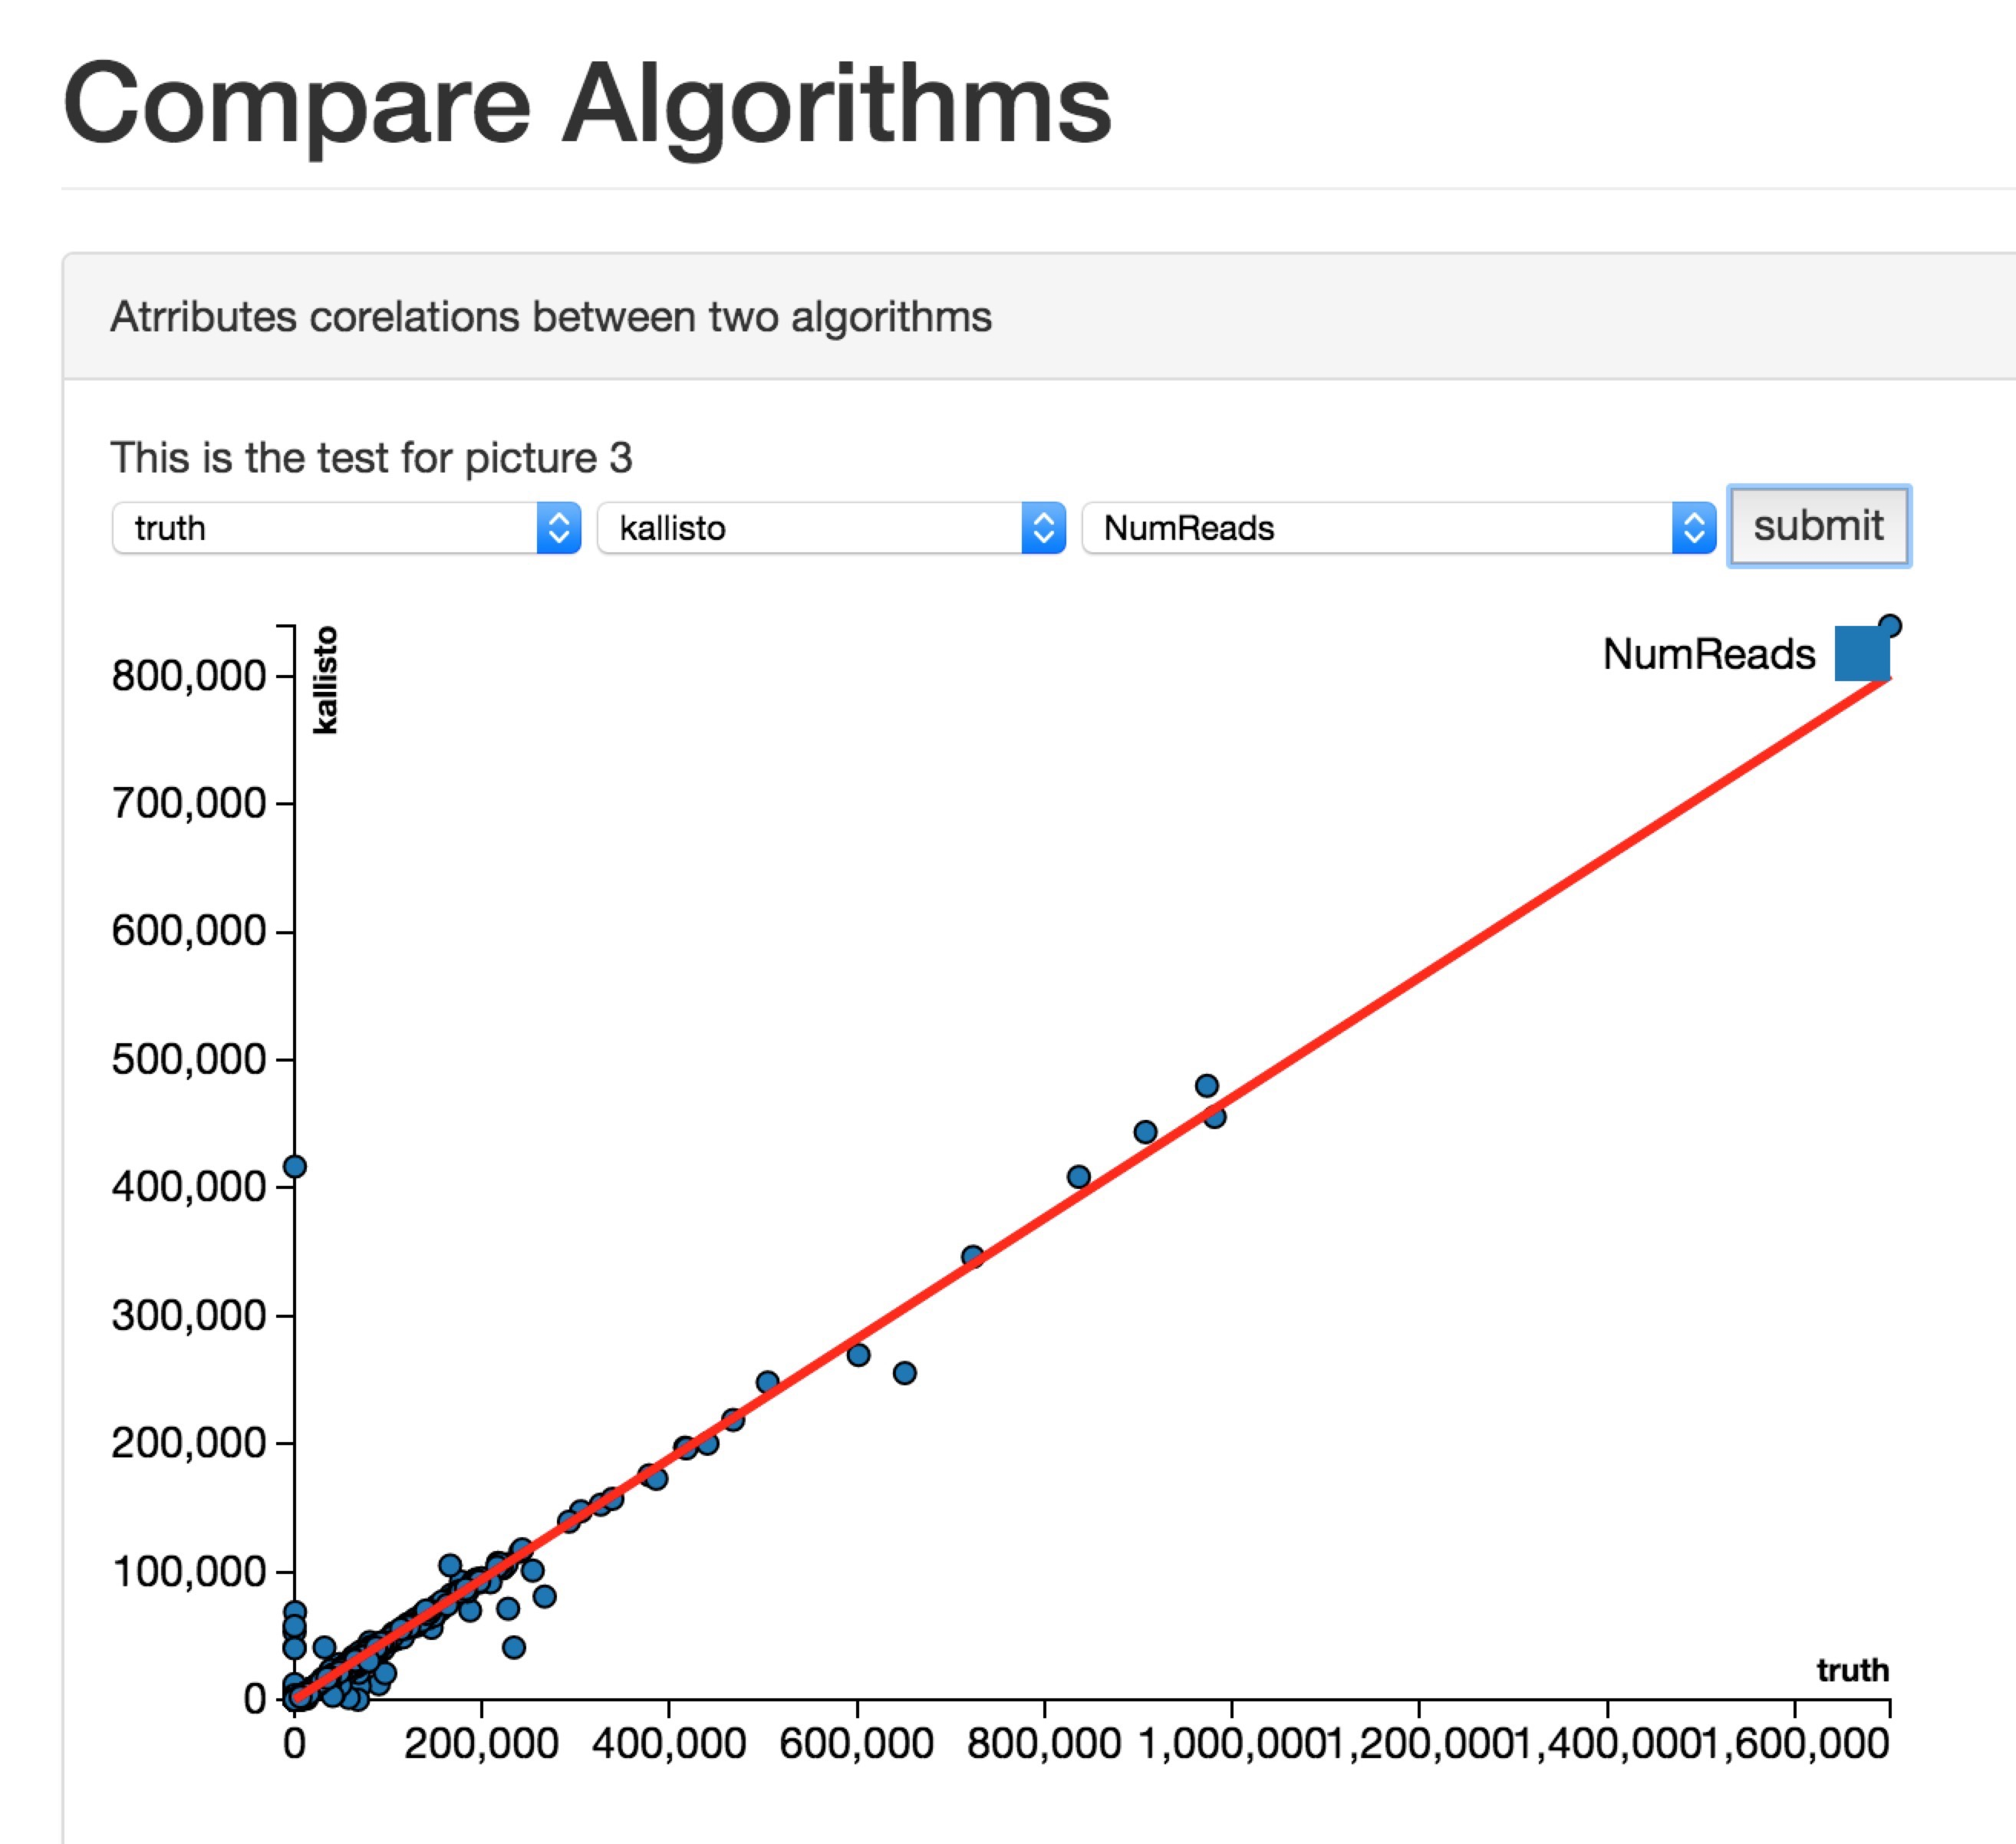
\includegraphics[height=2.5in, width=2.5in]{fig/compare_truth.jpg}
                \caption{Compare NumReads between ground truth and Kallisto  }
                \label{fig:compare_truth}
        \end{subfigure}
        \caption{Pictures of Clustering with Random Sampling}\label{fig:cluster}
\end{figure}

\subsection {Performance Evaluation}
We could also calculate the performance evaluation based on ground truth. The ground truth could be uploaded at upload page showed in figure \ref{fig:metrics}

\begin{figure}[h!]
\centering
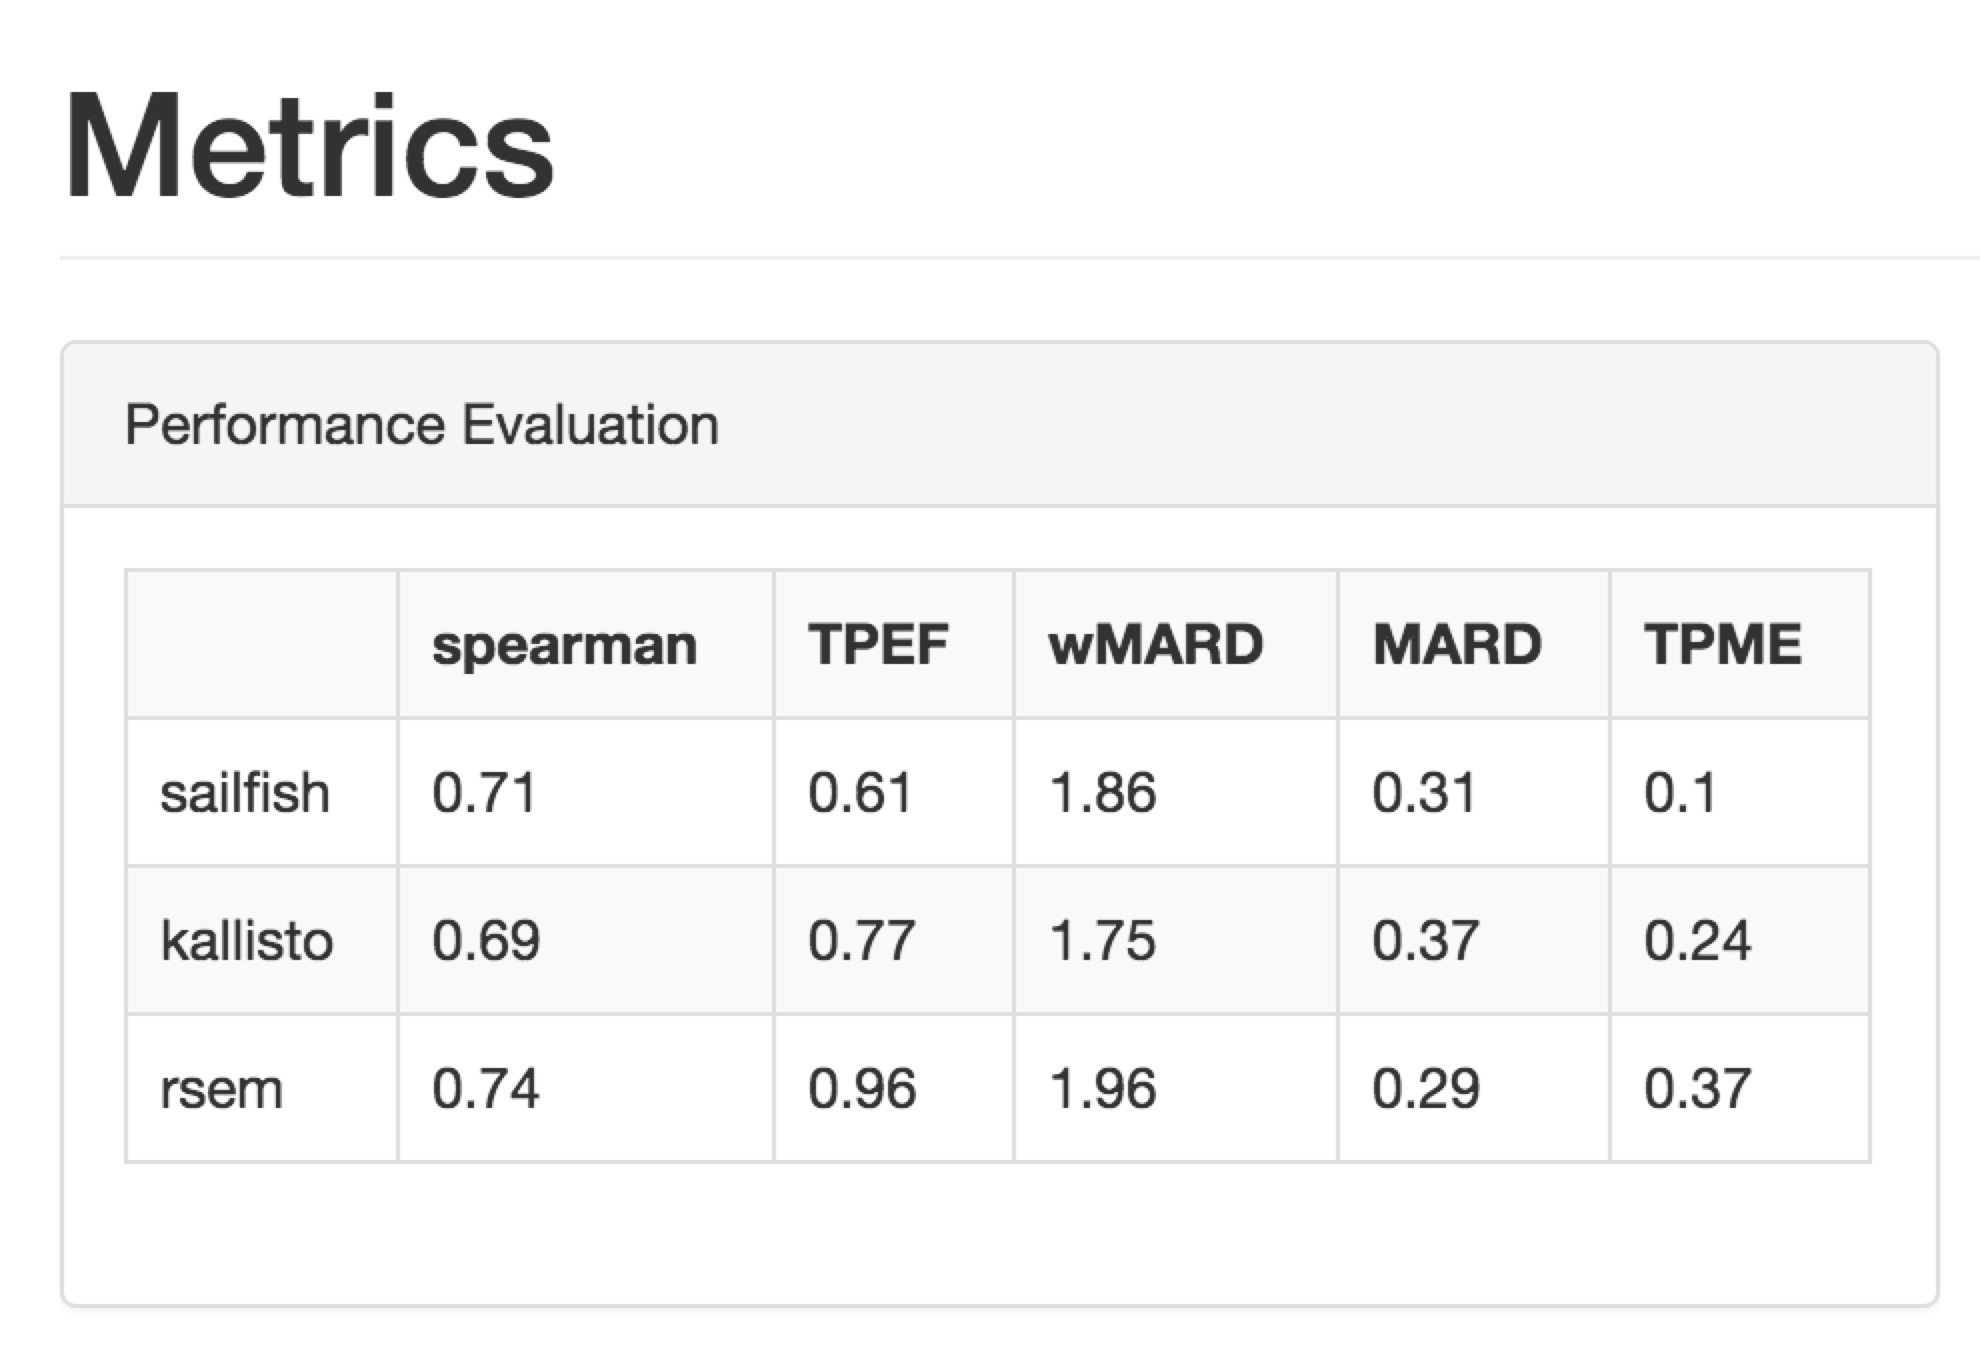
\includegraphics[height=2.25in, width=3in]{./fig/metrics.jpg}
\caption{Performance Evaluation}
\label{fig:metrics}
\end{figure}

By given the ground truth, we now could calculate the following metrics: Spearman corr., TPEF, TPME, MARD, wMARD \cite{rapmap}.


\section {Extensibility}
\subsection {Upload new data}
Currently the uploading of ground truth is added to re-calculate the performance evaluation results. \\
We also considered the extensibility in our implementation. Currently the result files are directly uploaded to the server side and by upload and rename to the targeted name, call $DataAnalyzor.load\_data()$, the server could reload all data to replace the old metrics. \\
Currently the filename for each algorithm is coded in $dataAnalyzor$'s constructor.
\subsection {Add new algorithm}
To add a new algorithm, one just need to add a related method in $AnalyzorBuilder$  with the corresponding result file, parsing method same as in file $ParsingUtility.py$ and the new algorithm could automatically be supported by the whole framework. \\
At both the front-end and back-end, the algorithms are queried from the $DataAnalyzor$. Once the algorithms and the corresponding methods for reading the data in, the new algorithm and the data would be showed as same as other old features.

\section{Improvement and Future Works}
We still have several unfinished features such as: \\
\begin{enumerate}
\item Add upload file feature at the website.
\item Automatically add new algorithms. Currently the algorithm parser has predefined columns. If the result files are using unique names, such as $NumReads$, we could automatically add new algorithms just by upload the result file.
\end{enumerate}


\section{Acknowledge}
Thanks and regards to Professor Rob Patro's lectures. We were inspired by the algorithms and the vivid examples. \\
Thanks and regards to the TA Hirak. He helped us a lot on the project.

% \bibliographystyle{plain}	% (uses file "plain.bst")
% \bibliography{literature}


% \section{References}
\begin{thebibliography}{100} % 100 is a random guess of the total number of
%references
\bibitem{sb_admin_2} "SB Admin 2 - Free Bootstrap Admin Theme." Start Bootstrap. N.p., n.d. Web. 15 Dec. 2015.\\ $<http://startbootstrap.com/template-overviews/sb-admin-2/>$.

\bibitem{d3_scatterplot}"D3 Scatterplot Example." D3 Scatterplot Example. N.p., n.d. Web. 15 Dec. 2015.\\ $<http://bl.ocks.org/weiglemc/6185069>$.

\bibitem{rapmap} Srivastava, Avi, Hirak Sarkar, and Rob Patro. "RapMap: A Rapid, Sensitive and Accurate Tool for Mapping RNA-seq Reads to Transcriptomes." \emph{bioRxiv} (2015): 029652.
\end{thebibliography}

% \input{appendix}

\end{document}
